\documentclass[8pt, landscape, fleqn]{scrartcl}
\setlength{\parindent}{0pt}
\usepackage[ngerman]{babel}
%\usepackage[applemac]{inputenc}
\usepackage[utf8]{inputenc}
\usepackage[dvips]{geometry}
\usepackage{latexsym}
\usepackage{multicol}
\usepackage{amsmath}
\usepackage{graphicx}
\usepackage{array}
\usepackage{booktabs}
\usepackage{amsmath}
\usepackage{mathtools}
\usepackage{ulem}
\usepackage{amsfonts}
\usepackage{dsfont}
\usepackage{charter} %%% Schreibart
%\renewcommand{\familydefault}{\sfdefault}



%%%%%%%%%%Paket für Chemische Formeln
\usepackage{chemformula} 
\usepackage[version=3]{mhchem}
%%%%%%%%%%%%%%%%% Farbe
\usepackage{color}

\pagestyle{plain}
\typearea{20}
\columnsep 30pt
\columnseprule .4pt
\setlength{\extrarowheight}{0.9em}

\renewcommand{\arraystretch}{0.8}

\makeatletter
\renewcommand{\section}{\@startsection{section}{1}{0mm}%
{-2\baselineskip}{0.8\baselineskip}%
{\hrule depth 0.2pt width\columnwidth\hrule depth1.5pt
width0.25\columnwidth\vspace*{1.2em}\Large\bfseries\rmfamily}}
\makeatother


\makeatletter
\renewcommand{\subsection}{\@startsection{subsection}{1}{0mm}%
{-2\baselineskip}{0.8\baselineskip}%
{\hrule depth 0.2pt width\columnwidth\hrule depth0.75pt
width0.25\columnwidth\vspace*{1.2em}\large\bfseries\rmfamily}}
\makeatother

\makeatletter
\renewcommand{\subsubsection}{\@startsection{subsubsection}{1}{0mm}%
{-2\baselineskip}{0.8\baselineskip}%
{\hrule depth 0.2pt width\columnwidth\vspace*{1.2em}\normalsize\bfseries\rmfamily}}
\makeatother

\newcommand{\Mx}[1]{\begin{bmatrix}#1\end{bmatrix}}
\begin{document}
\part*{\LARGE\textrm{Ausgewählte Kapitel der Flugtechnik $\hfill$ Xeno Meienberg}}
\begin{multicols*}{3}

\section{Flugtechnik}

\subsection{Atmosphäre}
\subsubsection{Allgemeine Eigenschaften}
Zusammensetzung: $\sim 78\% N_2$, $\sim 21\% O_2$, $ \sim 1\% He, H, He$
\newline \newline
\textbf{Troposphäre (0-7/17 km):} $\frac{dT}{dH} = -6.5\cdot 10^{-3} \frac{K}{m}$ \newline In ihr findet das Wetter statt
\newline \newline
\textbf{Tropopause (abhängig von Breitengrad und Jahr)}: \newline
"Aquator (17 km): $T = 191 K$ \newline 
Pole (7km): $T = 221 K$
\newline \newline
\textbf{Standardatmosphäre (11 km)}: $T_{11000} = 216.65 K$, $p_{11000} = 226.32 HPa$, $\rho_{11000} = 0.3639 km/m^3$
\newline \newline
\textbf{Stratosphäre (bis $\sim$ 50 km)}: $T = 217 K$ (direkt "uber Tropopause, max. bei 50 km)
\newline \newline
\textbf{Stratopause ($\sim$ 50 km)}: $T = 273 K$
\newline \newline
\textbf{Mesosphäre (bis $\sim$ 80 km)}: $T = 173 K$ (negativer Temp. gradient)
\newline \newline
\textbf{Thermosphäre und Ionosphäre (bis $\sim 800km$)}: $T = 1270 K$ bei $480 km$
\newline \newline
\textbf{Exosphäre (ab $800 km$)}: Führt gleitend in den Weltall
\newline \newline
\textbf{Physikalischen Eigenschaften}:
\begin{itemize}
\item $p = \rho R T$ mit $R = 287.3 J/(kg K)$ 
\item Bernoulli: $p + \frac{\rho}{2}V^2 = const$
\item Schallgeschwindigkeit: $a = \sqrt{\gamma R T}$ mit $\gamma = c_p / c_v$
\item Luft: $\gamma = 1.405$
\item $\frac{\Delta \rho}{\rho} \approx \frac{1}{2} M^2$, Machzahl $M = V/a$
\end{itemize}

\subsection{Standardatmosphäre}
\begin{itemize}
    \item $H = 0m$
    \item $T_0 = 288.15 K$, $p = 1013 HPa$, $\rho = 1.225 kg/m^3$, $g = 9.806 m/s^2$
    \item $H < 11000 m$
    \item $\frac{T}{T_0} = \Theta(H)= 1 + \frac{a}{T_0} H = 1-22.558\cdot 10^{-6} \cdot H$
    \item $\frac{p}{p_0} = \delta = \Theta^{5.2561}$
    \item $\frac{\rho}{\rho_0} = \sigma = \Theta^{4.2561}$
    \item $H = 11000 m$:
    \item $\frac{T_{11000}}{T_0} = 0.7519$, $\frac{p_{11000}}{p_0} = 0.2234$, $\frac{\rho_{11000}}{\rho_0} = 0.2971$
    \item $11000 m < H < 25000m$: 
    \item $\frac{T}{T_0}= 0.7519$, $\frac{p}{p_0} = 0.2234 \cdot e^{-\frac{H-11000}{6341.9}}$, $\frac{\rho}{\rho_0} = 0.2971 \cdot e^{-\frac{H-11000}{6341.9}}$
    \item Dynamische Zähigkeit der Luft:
    \item $\mu = (1.458\cdot 10^{-6}\cdot T^{1.5})/(T+110.4) Ns/m^2$
    \item $\mu_0 = 17.894 \cdot 10^{-6} Ns/m^2$
    \item Kinematische Viskosität: $\nu = \mu / \rho~ [m^2/s]$ 
\end{itemize}

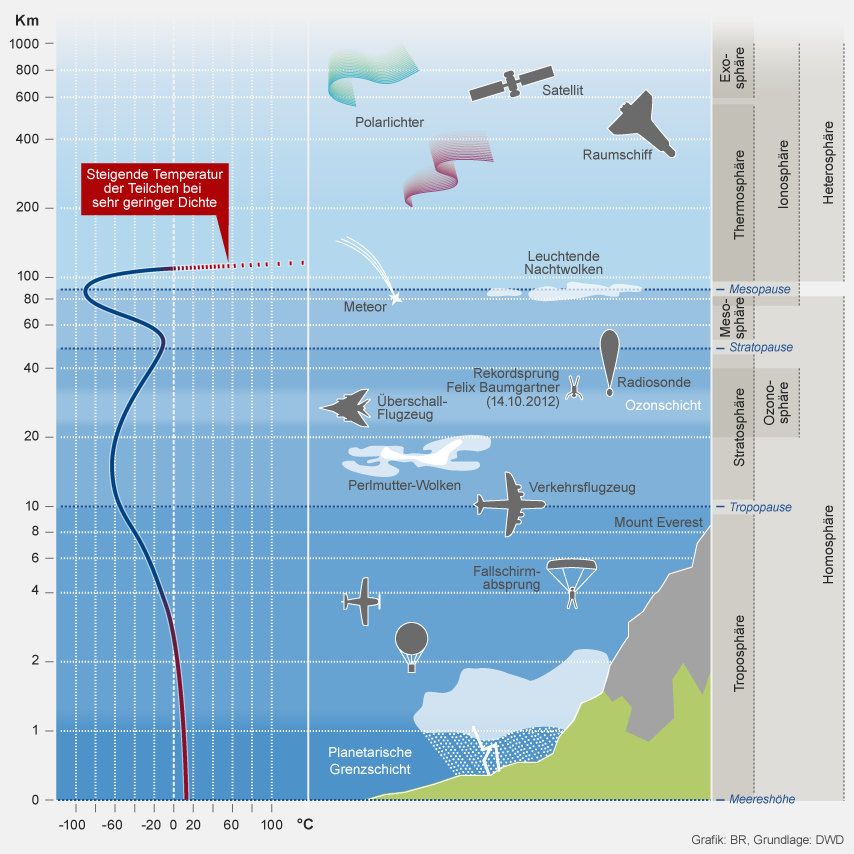
\includegraphics[width=8cm]{images/meteorologie-wetter-atmosphaere-102}

\subsection{Auftrieb}
\subsubsection{Flügelgeometrie}

\begin{itemize}
    \item Zuspitzung: $\lambda = \frac{c_t}{c_0}$
    \item Flügelfläche: $F = \int_{-b/2}^{b/2} c(y) dy$ 
    \item Streckung: $\Lambda = b^2 /F$
    \item Mittl. geome. Flügeltiefe: $\overline{c} = \frac{1}{b} \int_{-b/2}^{b/2} c(y) dy = F/b$ 
    \item Mittl. aero. Flügeltiefe: $l_\mu = \frac{1}{F} \int_{-b/2}^{b/2} c^2(y) dy $
    \item Geometrischer Neutralpunkt = Ort wo die Änderung des Anstellwinkels keine Auswirkung auf Kraft und Moment hat
    \item $x_{N25} = \frac{1}{F} \int_{-b/2}^{b/2} c^2(y) x_{25}(y) dy \approx x_{c_0/4}$, $y_{N25} = 0$
\end{itemize}

Achtung: $b_{ges} = 2\cdot b_{flugel}$!

\begin{center}
    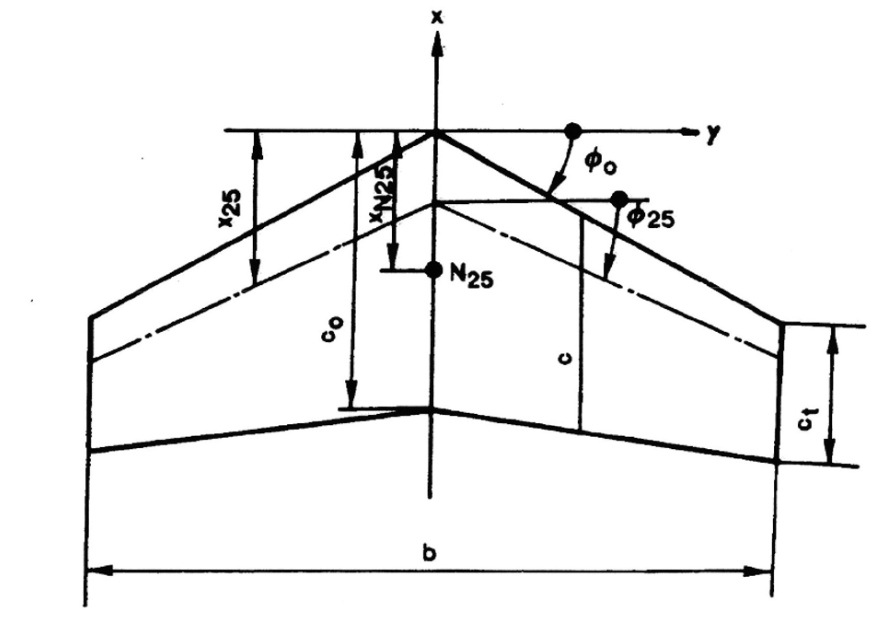
\includegraphics[width = 6cm]{images/Fluegelgeometrie-1.png}
\end{center}
\begin{tabular}{ l | l l l l}
    & Recht & Trapez & Dreieck & Ellipse \\ 
    \hline
    F & $bc$ & $\frac{c_0+c_t}{2}b$ & $\frac{c_0}{2}b$ & $\frac{\pi}{4}b c_0$ \\ 
    \hline 
    $\Lambda$ & $b/c$ & $2b/(c_0+c_t)$ & $2b/c_0$ & $4b/(\pi c_0)$ \\
    \hline
    $\lambda$ & $1$ & $c_t/c_0$ & 0 & - \\
    \hline
    $\overline{c}$ & c & $(c_0+c_t)/2$ & $c_0/2$ & $\pi/4$ \\
    \hline
    $l_\mu$ & c & $\frac{2}{3}\frac{c_0^2+c_0c_t+c_t^2}{c_0+c_t}$ & $2c_0/3$ & $\frac{8}{3\pi}c_0$ \\
    \hline
    $x_{25}$ & $c/4$ & $\frac{c_0}{4}+\frac{c_0 b}{6(c_0+c_t)}(1+\frac{2c_t}{c_0})tg(\phi_{25})$ & $\frac{c_0}{4}\frac{b}{6}tg(\phi_{25})$ & $\frac{c_0}{4}\frac{b}{6}tg(\phi_{25})$ \\
    \hline
\end{tabular}

\subsubsection{Flügelprofile}

\begin{tabular}{l | l l }
    & Flügel (3D) & Profil (2D) \\ 
    \hline
    Auftrieb & $c_A = \frac{A}{\frac{1}{2}\rho V^2 F}$& $c_a = \frac{A'}{\frac{1}{2}\rho V^2 c}$  \\
    \hline
    Widerstand & $c_W = \frac{W}{\frac{1}{2}\rho V^2 F}$ & $c_w = \frac{W'}{\frac{1}{2}\rho V^2 c}$ \\
    \hline
    Nickmoment & $c_M = \frac{M}{\frac{1}{2}\rho V^2 F l_\mu}$ & $c_m = \frac{M'}{\frac{1}{2}\rho V^2 c^2}$\\
    \hline
\end{tabular}
\newline \newline
Hierbei sind Grössen mit Apostroph pro Spannbreite berechnet (Kraft/Moment pro $b$)

\begin{itemize}
    \item \textbf{Auftriebspolaren:} Nullauftriebswinkel $\alpha_0$ (Winkel wo aerodyn. Auftrieb verschwindet)
    \item $\alpha_0 = 0$ für symmetrische Profile
    \item $\alpha_0 < 0$ für gewölbte Profile
    \item \textbf{Linearbereich}
    \item $c_a = \frac{dc_a}{d\alpha}(\alpha-\alpha_0)$ mit Auftriebsgradient 
    \item $\frac{dc_a}{d\alpha}$: Konstant im Linearbereich
    \item \textbf{Maximaler Auftriebsbeiwert:} $c_{a,max}$ bestimmt die Abrissgeschwindigkeit
    \item \textbf{Minimaler Auftriebsbeiwert:} $c_{a,min}$ analog wie $c_{a,max}$ im Rückenflug
    \item \textbf{Minimaler Widerstandsbeiwert:} $c_{w,min}$ 
    \item $c_{w,min} = 0$ für symmetrische Profile
    \item $c_{w,min} > 0$ für gewölbte Profile ungefähr beim stossfreien Eintritt (tangentialle Umströmung)
    \item \textbf{Sturzflug-Momentenbeiwert} $c_{m_0} = c_m(c_a = 0)$
    \item \textbf{Bester Gleitwinkel}: $\tan(p) = \frac{1}{(\frac{c_a}{c_w})_{max}}$
    \item \textbf{Grössmögliche Reichweite:} $(\frac{c_a}{c_w})_{max}$
    \item \textbf{Beste Steigzahl / Profilsinkzahl:}
    \item $(\frac{c_a^3}{c_w^2})_{max}$ resp. $\sqrt{\frac{c_a^3}{c_w^2}}$ längste Flugdauer 
\end{itemize}

\begin{center}
    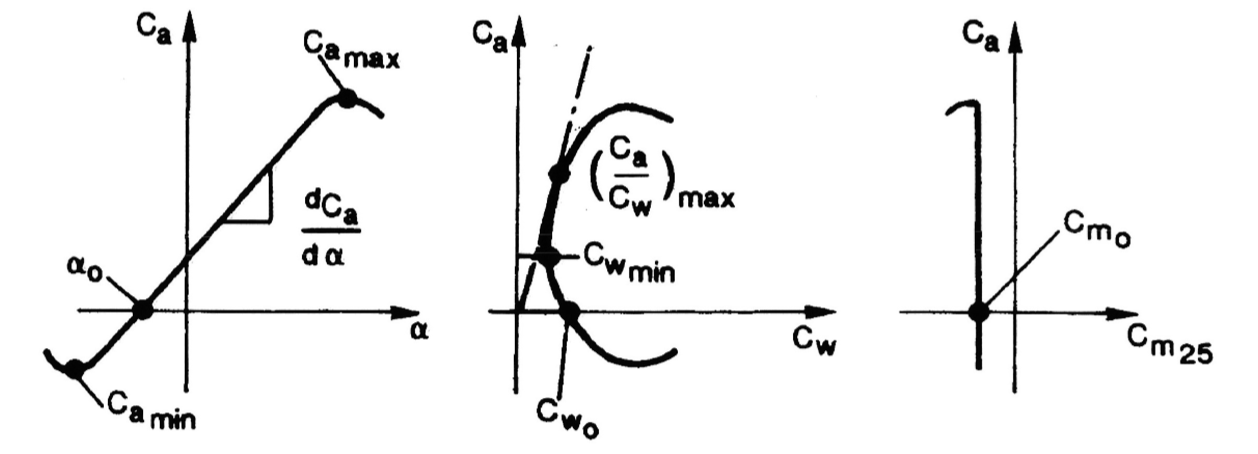
\includegraphics[width = 8cm]{images/Aufstiegspolaren.png}
\end{center}

\begin{itemize}
    \item \emph{Druckpunkt / Neutralpunkt}
    \item Druckbeiwert: $c_p = \frac{p-p_\infty}{1/2 \rho V^2}$
    \item Moment um beliebigen Punkt am Profil:
    \item $c_{m_x}= \frac{x-x_{DP}}{c}(c_a \cos\alpha + c_w \sin\alpha) \approx \frac{x-x_{DP}}{c}c_a$
    \item $x_{DP}$: Lage des Druckpunktes
    \item Am \textbf{Druckpunkt}: $c_{m,DP} = 0$
    \item \textbf{Neutralpunkt}: $\frac{dc_{m_x}}{d\alpha}\vert_{NP} = 0$ und $\frac{dc_{m_x}}{dc_a}\vert_{NP} = 0$
    \item $\frac{x_{NP}-x_R}{c} = -\frac{c_{mR}-c_{m0}}{c_a}$ mit $R$ als Referenzpunkt
\end{itemize}

\subsubsection{Profileigenschaften}

\begin{itemize}
    \item Auftrieb [N/m]: $A= \rho V\Gamma$ 
    \item Zirkulation $[m^2/s]$: $\Gamma = \int_0^c \gamma dx~ [m^2/s]$
    \item \textbf{Einwirbel-Modell}
    \item $A = \rho V^2 \pi c \alpha$, $\frac{dc_a}{d\alpha} = 2\pi$, $c_a = 2\pi\alpha$                                                                                                                                                                                             
\end{itemize}

\subsubsection{Profilsystematik siehe p. 3.34}

\subsubsection{Tragflügel endlicher Spannweite}

\textbf{Aerodynamische Kraft auf Flügel}

\begin{itemize}
    \item $A = \int_{-b/2}^{b/2} \rho V \Gamma(y) dy$
\end{itemize}

\textbf{Induzierter Widerstand}




\begin{itemize} 
    \item $W_i = \frac{A^2}{2\rho V^2F^*} = \frac{2}{\rho V^2 \pi}\left(\frac{A}{b}\right)^2$
    \item mit Prandtl'schem Ansatz $F^* = \frac{\pi}{4}b^2$
    \item $c_{w_i} = \frac{c_a^2}{\pi \Lambda}$ und $\alpha_i = \frac{c_a}{\pi \Lambda}$
\end{itemize}

\textbf{Einfaches Wirbelmodell (Hufeisenwirbel)}

\begin{itemize}
    \item Abwind im Hufeisenwirbel mit $-x \gg y$
    \item $w = w_{re}+ w_{li} = \frac{\Gamma}{2\pi}\left(\frac{1}{b/2-y}+\frac{1}{b/2+y}\right)$
    \item Abwind im Hufeinsenwirbel auf Flügellinie
    \item $w = w_{re}+ w_{li} = \frac{\Gamma}{4\pi}\left(\frac{1}{b/2-y}+\frac{1}{b/2+y}\right)$
    \item Auftrieb über ganze Spannweite
    \item $A = \rho V \Gamma b$
\end{itemize}
\textbf{Allgemeine induzierte Geschwindigkeit}
\begin{itemize}
    \item Halbunendlicher Wirbelfaden: $w_i = \frac{\Gamma}{4\pi a}$
    \item Unendlicher Wirbelfaden: $w_i = \frac{\Gamma}{2\pi a}$
\end{itemize}

\begin{center}
    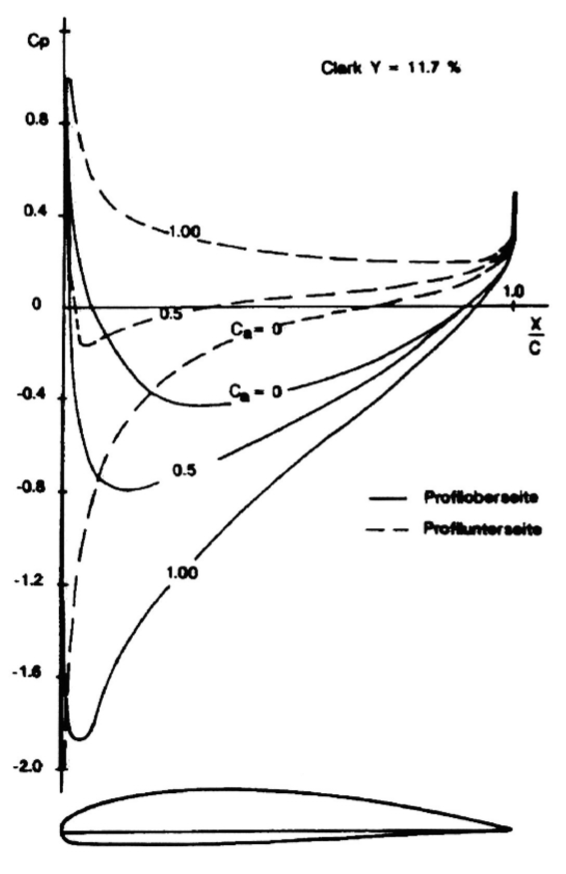
\includegraphics[width = 5.5cm]{images/Druckverteilung_am_Profil.png}
\end{center}


\subsubsection{Prandtl'sche Traglinientheorie}
Zirkulationsverteilung für \textbf{elliptische Auftriebsverteilung}
\begin{itemize}
    \item $\Gamma(y) = \Gamma_0 \sqrt{1-\left(\frac{2y}{b}\right)^2}$, ind. Anstellwinkel: $\alpha_i = \frac{\Gamma_0}{2bV}$
    \item Elliptische Flügel erzeugen ... eine elliptische Auftriebsverteilung 
    \item ... einen in Spannweitenrichtung kontanten Abwind
    \item ... in Spannweitenrichtung konstanten lokalen Auftriebsbeiwert
    \item $\alpha_i = \frac{c_A}{\pi \Lambda}$ Abwindwinkel des Ellipsenflügels am Flügel selbst
    \item $c_A = c_{a_\alpha}\frac{\Lambda}{\Lambda+2}\alpha~$ Auftriebsbeiwert des Ellipsenflügels
    \item $\frac{d c_A}{d \alpha} = c_{a_\alpha}\left[\frac{1}{1+\frac{c_{a_\alpha}}{\pi \Lambda}}\right]$ Auftriebsderivativ des Ellipsenflügels
    \item $\frac{d c_A}{d \alpha} = c_{a_\alpha}\frac{\Lambda}{\Lambda+2}$ Auftriebsderivativ des Ellipsenflügels (potentialtheoretisch)
    \item $c_{W_i}=\frac{c_A^2}{\pi \Lambda}$ Induzierter Widerstand des Ellipsenflügels
\end{itemize}
\textbf{Beliebige Auftriebsverteilung}
\begin{itemize}
    \item \emph{Methode von Schrenk}: Aufteilung von Auftriebsverteilung auf Basisauftrieb und Zusatzauftrieb (A/2 elliptische Form, A/2 proportional zu Flügelgrundriss)
    \item $\frac{dc_A}{d\alpha} = c_{a_\alpha}\left[\frac{\Lambda}{\Lambda+\frac{2(\Lambda+4)}{\Lambda+1}}\right]$ (McCormick Näherung)
    \item $\frac{dc_A}{d\alpha} = c_{a_\alpha}\left[\frac{\Lambda}{\frac{c_{a_\alpha}}{\pi}+\sqrt{\left(\frac{c_{a_\alpha}}{\pi}\right)^2+\Lambda^2}}\right]$, falls $c_{a_\alpha} = 2 \pi $:
    \item $\frac{dc_A}{d\alpha} = c_{a_\alpha}\frac{\Lambda}{2+\sqrt{4+\Lambda^2}}$ (Lowry+Polhermus Näherung)
\end{itemize}

\begin{center}
    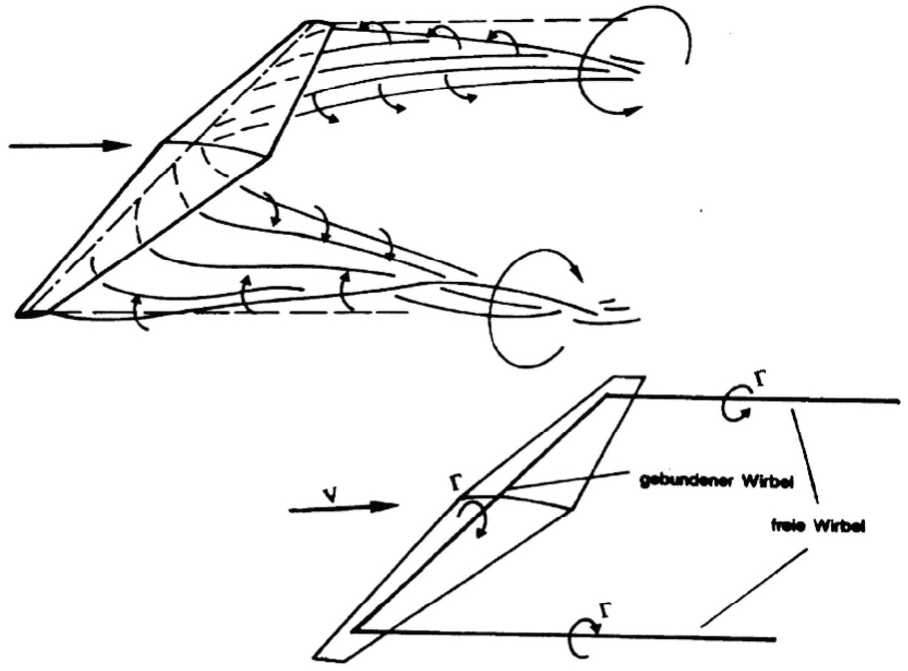
\includegraphics[width=5.5cm]{images/Wirbelsystem_einfaches_Hufeisenmodell.png}
    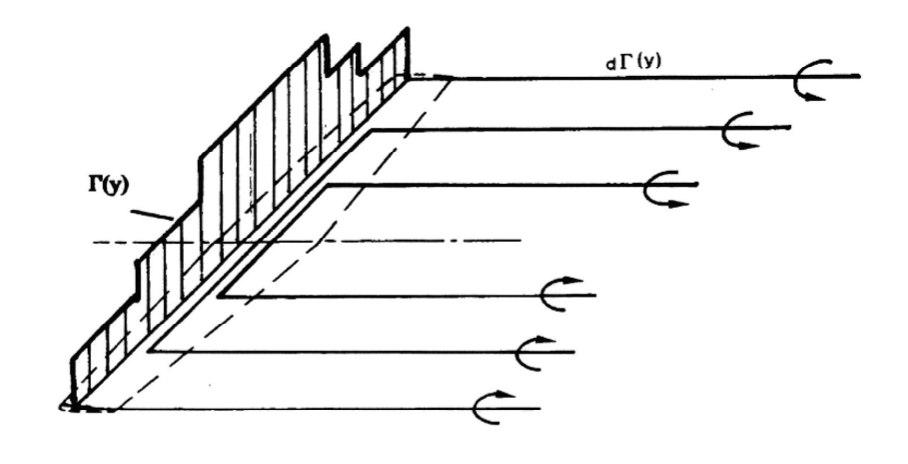
\includegraphics[width=5.5cm]{images/Prandtl_Wirbelmodell.png}
\end{center}

\textbf{Prandtl-Glauert Faktoren}

\begin{itemize}
    \item Prandtl-Glauert Faktoren $\tau$ und $\delta$ geben Abweichungen zum idealen Ellipsenflügel an 
    \item $\alpha_i = \frac{c_A}{\pi A}(1+\tau)$
    \item $c_{W_i} = \frac{c_A^2}{\pi A}(1+\delta)$
\end{itemize}

\subsubsection{Strömungsabriss am Flügel}
\begin{itemize}
    \item Abbrissverhalten kritischer je ausgeprägter der Auftriebsabfall nach erreichen von $c_{A,max}$
    \item Abriss bemerkbar durch Schütteln (Buffeting)
    \item Abriss erkennbar wenn Innenflügel im abgerissenen Zustand und Aussenflügel gesund umströmt
    \item Bei Trapezflügel: Abrissverhalten aussen kritischer
    \item Bei gepfeilter Flügelform: Zusätzlich kan ein Längsmoment (Pitch Up) eintreten, was zu einer Verstärkung des Abriss führt
    \item \textbf{Flügelverwindung}: Aeroelastische Antwort wobei Flügel nach aussen unten verwunden werden (-3°) damit Pilot länger Kontrolle auf Steuerruder hat
    \item \textbf{Stall Control Devices}:
    \item Absenkung der Profilnase im Ausenflügel (Drop Nose)
    \item Nasenklappen im Aussenflügel
    \item Sägezahn (bei Pfeilflügeln) zwecks Aufbau einer Grenzschicht
    \item Grenzschichtzaun, verhindert Strömungsabfluss gegen Flügelspitze
    \item Vortex-Generatoren, verzögern Ablösung im Querruder
    \item Abrisskanten (Stall Strips) am Innenflügel, lösen früher ab, Pilot wird durch Buffeting gewarnt ohne das Querruderwirksamkeit verloren geht
\end{itemize}



\subsubsection{Auftriebserhöhende Klappen}

\begin{itemize}
    \item Schnellflug: $c_{W,min}$ möglichst klein
    \item Reiseflug: $c_a/c_w$ resp. $c_a^3/c_w^2$ möglichst gross
    \item Langsamflug $c_{A,max}$ möglichst gross
    \item Um alle Anforderungen zu erfüllen, werden Klappen gebraucht
    \item Die Profilwölbung führt zu einem grösseren $c_{A,max}$ 
    \item $\frac{dc_a}{d\alpha}$ bleibt ungefähr gleich
    \item $c_a$ verschiebt sich zu grösseren Auftriebsbeiwerten
\end{itemize}


\subsection{Widerstand}

\subsubsection{Widerstandsarten}

\begin{center}
    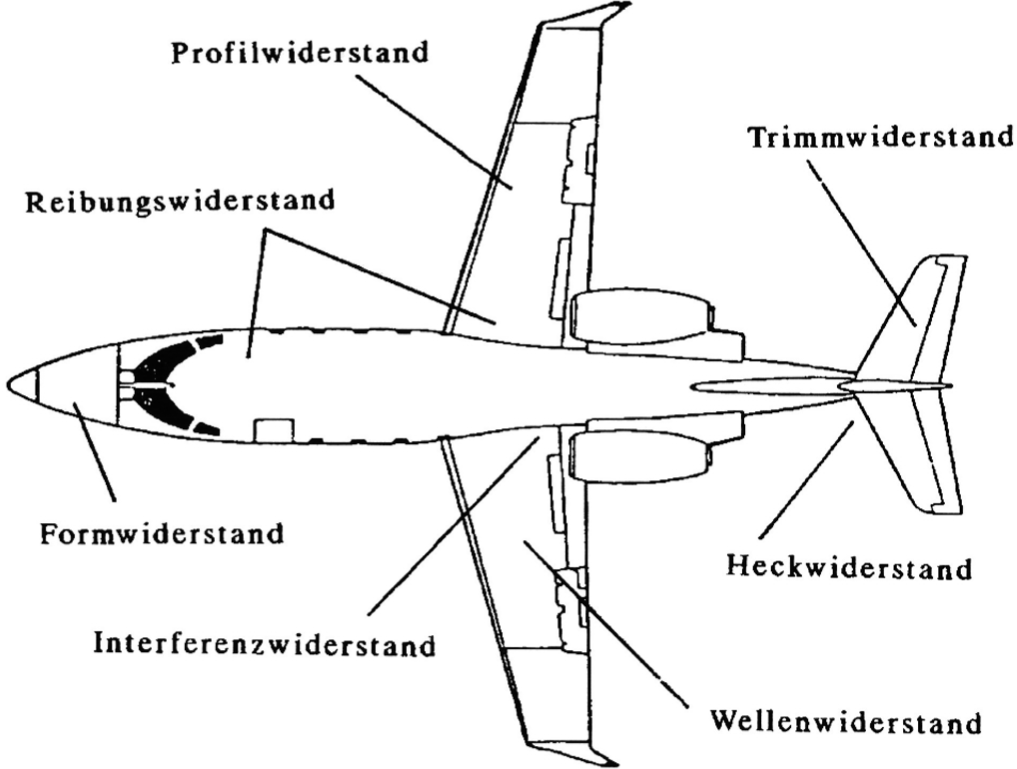
\includegraphics[width=6cm]{images/Widerstandsarten.png}    
\end{center} 

\textbf{Gesamtwiderstand = Induzierter Widerstand + Restwiderstand} \newline \newline
\textbf{Restwiderstand}
\begin{itemize}
    \item Reibungswiderstand: Reibungswiderstand auf benetzter Oberfläche
    \item Formwiderstand: Druckwiderstand auf Oberfläche parallel zur Strömung
    \item Interferenzwiderstand: Widerstand durch zwei Körper nahe beieinander
    \item Trimmwiderstand: Zusatzwiderstand durch Komponenten welche zum Momentengleichgewicht benötigt sind
    \item Profilwiderstand: Reibungs- und Formwiderstand eines 2-D Profils
    \item Kühlungswiderstand: Widerstand durch Impulsverlust beim Durchströmen von Kühleinrichtungen
    \item Heckwiderstand: Druckwiderstand eines stumpfen Hecks 
    \item Wellenwiderstand: Bei Überschallströmungen, durch Schockwellen
\end{itemize}

\textbf{Induzierter Widerstand}
\begin{itemize}
    \item $c_W = c_{W_0} + c_{W_i}$ wobei $c_{W_i} = kc_A^2$ (elliptisch: $k = \frac{1}{\pi \Lambda}$)
    \item $W = \frac{\rho}{2} V^2 F c_{W_0} + \frac{\rho}{2}V^2Fkc_A^2$ (dimensionsbehafte Form)
    \item Stationärer Horizontalflug ($A = mg$ und $c_A = \frac{2mg}{\rho V^2 F}$ )
    \item $W = \frac{\rho}{2} V^2 F c_{W_0} +  \frac{k(mg)^2}{\frac{\rho}{2}V^2F}$
\end{itemize}

\subsubsection{Restwiderstand des Flügels}
\textbf{Profilwiderstand}(Widerstand des Flügels) - p. 4.47 ff 


\begin{itemize}
    \item $W_{Fl"ugel} = W_{Rest,Fl} + W_{induziert}$
    \item $W_{Rest,Fl} = 2 \frac{\rho}{2}V^2 \int_{b_R/2}^{b/2} c_{W_\infty}(y)c(y)dy$  
    \item $c_{W_\infty}$ Profilwiderstand 2D
\end{itemize}

Unverwundener Ellipsenflügel:

\begin{itemize}
    \item $W_{Fl"ugel} = c_{W_\infty} \frac{F^*}{F}+c_{W_i}$ 
    \item $F^*$ benetzter Anteil Flügelfläche
\end{itemize}

Oswald-Faktor

\begin{itemize}
    \item $c_W = c_{W_0}+ \frac{c_A^2}{\pi \Lambda e}$ mit 
    \item $e = \frac{1}{1+\delta+\pi\Lambda k}$ Oswald-Wirkungsfaktor
    \item Gilt nur im Linearbereich der Auftriebspolaren!
    \item Flügel mit elliptischer Auftriebsverteilung: $e=1$
    \item Flügel $0.85<e<0.95$
    \item Flugzeug $0.6<e<0.9$
\end{itemize}

Bester Gleitwinkel $(c_A/c_W)_{max}$

\begin{itemize}
    \item $c_W = 2c_{W_0}$, $c_A = \sqrt{\pi \Lambda e c_{W_0}}$, $c_{W_0} = c_W(c_A = 0)$
\end{itemize}

\subsubsection{Restwiderstand des Flugzeugs}

\textbf{\emph{Reibungswiderstand} $W_R$}

\begin{itemize}
    \item $c_f = \frac{W_R}{\frac{\rho}{2}V^2F_W}$ mit $F_W$: benetzte (überstr.) Oberfläche
    \item Lokale Reynoldszahl: $Re_x = \frac{V x}{\nu}$
\end{itemize}

\textbf{Umschlag von laminar-turbulent}

\begin{itemize}
    \item $Re_{krit} = (V x / \nu)_{krit} \approx 3\cdot 10^5-3\cdot 10^6$
    \item laminar $Re < Re_{krit}$
    \item turbulent $Re > Re_{krit}$
\end{itemize}

\textbf{Ebene Platte mit glatter Oberfläche}

\begin{itemize}
    \item $Re = (V l /\nu) $ mit $l$ Plattenlänge
    \item laminar: $c_f = 1.328 \frac{1}{\sqrt{Re}}$
    \item turbulent: $c_f = 0.074 Re^{-1/5}$
\end{itemize}

\textbf{Ebene Platte mit rauher Oberfläche}
\newline Rauhigkeit $k_s$
\begin{itemize}
    \item $k_s = 0 mm$ - Aerodynamisch/hydraulisch glatt
    \item $k_s = 0.5\cdot10^{-3} - 2 \cdot 10^{-3} mm $ - Metall/Holz poliert 
    \item $k_s = 6\cdot 10^{-3} mm$ - Farboberfläche, glänzend
    \item $k_s = 0.01-0.03 mm$ - Tarnfarbe, unpoliert
    \item $k_s = 0.15 mm$ - Metalloberfläche, galvanisierend
\end{itemize}
Rauhigkeitsbereiche:
\begin{itemize}
    \item $\frac{u_\tau k_s}{\nu} < 5$ hydraulisch glatt
    \item $5 <\frac{u_\tau k_s}{\nu} < 70$ Übergangsbereich
    \item $\frac{u_\tau k_s}{\nu} > 70$ rauh 
\end{itemize}
Zulässige Rauhigkeitshöhe $k_{s,zul}$ für Grenzschichten
\begin{itemize}
    \item laminare GS: $k_{s,zul} \leq 15 \frac{u_\tau}{\nu} = k_{s,krit} = 26.03 \frac{\nu \sqrt[4]{Re_x}}{V}$
    \item turbulente GS: $k_{s,zul} < 100 \frac{\nu}{V} = 100 \frac{l}{Re}$
    \item $c_f = (1.89 + 1.62 \log(\frac{1}{k_s}))^{-2.5}$ für $10^2 < \frac{1}{k_s} < 10^6$
\end{itemize}

\textbf{Plattenförmige Körper ohne grosse Ablösungssgebiete}

\begin{itemize}
    \item $c_W^* = c_f \frac{F_W}{F_F}$
    \item Benetzte Oberfläche $F_W$, Frontfläche $F_F$
\end{itemize}

\textbf{Reibungswiderstand für profilierte Flächen (empirische Beziehung)}

\begin{itemize}
    \item $c_{W_0} = c_f \frac{F_F}{F}\left[1 + L\left(\frac{d}{c}\right)+100\left(\frac{d}{c}\right)^4\right]$
    \item mit $L = 1.2$: Falls Profil max. Dicke $x/c > 0.3$
    \item mit $L = 2.0$: Falls Profil max. Dicke $x/c < 0.3$
    \item $F$: Referenzfläche, $F_W$: Benetzte Oberfläche
    \item $c$: Profiltiefe, $d$: Profildicke
\end{itemize}

\textbf{Formwiderstand}

\begin{itemize}
    \item $c_{W,Ru}(\alpha) = c_{W_{0,Ru}}+c_{W_{\alpha,Ru}}+c_{W_{H,Ru}}$
    \item $c_{W,Ru} = 0.05-0.15$ \newline $0.15$ für kleine, gedrungene Flugzeuge
    \item $c_{W,Ru} = \left( 1 + \frac{D}{2l}\right)c_{f,pl}\frac{F_W}{F}$ \newline $c_{f,pl}$ Reibungsbeiwert Platte
    \item $c_{\alpha,Ru} \approx k_R \left(\frac{\alpha}{10}\right)^3 c_{W_{0,Ru}}$ \newline $k_R \approx 0.3$ (gedrungen), $k_R \approx 0.9$ (schlank)
    \item $c_{W_{H,Ru}} = 0.029 \left(\frac{D_H}{D}\right)^3 \frac{1}{\sqrt{c_{W_{0,Ru}}}}\frac{\pi D^2}{4}\frac{1}{F}$ \newline $D$: max. Rumpfdurchmesser, $D_H$: Heckdurchmesser
\end{itemize}

\textbf{Interferenzwiderstand}

\begin{itemize}
    \item $\approx 5\%$ des Rumpfwiderstands bei kleinen Anstellwinkeln, durch Messungen zu bestimmen
\end{itemize}

\textbf{Trimmwiderstand}

\begin{itemize}
    \item $\approx max. 1-2 \%$ des Gesamtwiderstands im stationären Reiseflug
\end{itemize}

\textbf{Abschätzung des Restwiderstands}

\begin{enumerate}
    \item Einzelteile auflisten
    \item Geometrie der Einzelteile bestimmen
    \item Referenzfläche $F_N$ bestimmen und Widerstandsbeiwert $c_{W_n}$ abschätzen
    \item Widerstandsfläche der Einzelteile berechnen: $f_n = c_{W_n}F_n$
    \item Widerstandsfläche des Flugzeugs bestimmen: $f = \sum_{i=1}^n f_i$
    \item Abschätzen von allfälligen Zusatzwiderständen (Interferenzen, Kühlung)
    \item Gesamtwiderstand: $W_{Rest} = \frac{1}{2}\rho V^2 f +W_{zusatz}$
\end{enumerate}

\subsubsection{Gesamtwiderstand des Flugzeugs}

\begin{itemize}
    \item $W = \frac{1}{2}\rho V^2 \left(f + F \frac{c_A^2}{\pi \Lambda e}\right)$
    \item Im stationären Horizontalflug: $A = mg$
    \item $W = \frac{1}{2}\rho V^2 f + \frac{2}{\rho \pi e}\left(\frac{mg}{b}\right)^2\frac{1}{V^2}$
\end{itemize}

\textbf{Minimaler Widerstand}

\begin{itemize}
    \item $W_{min} = \frac{2mg}{b}\sqrt{\frac{f}{\pi e}}$
    \item $V(W_{min}) = \left[\frac{4}{\pi e f}\left(\frac{mg}{\rho b}\right)^2\right]^{0.25}$
\end{itemize}

\subsubsection{Widerstandsverminderung}

\textbf{Reduktion des induzierten Widerstands}

\begin{itemize}
    \item $c_{W_i} = \frac{c_A^2}{\pi \Lambda e} \rightarrow$ möglichst grosse Streckung $\Lambda$
    \item Möglichst elliptischer Auftrieb $e = 1$
    \item Durch Beeinflussung der Ausgleichsströmung (Flügelend-Tanks, Winglets etc.)
\end{itemize}

\textbf{Reduktion des Restwiderstand (p. 4.36)}

\begin{itemize}
    \item Reduktion der Oberflächenreibung durch Laminarhaltung der Strömung
    \item Reduktion der Oberflächenreibung durch Reduktion der Rauheit 
    \item Grenzschichtbeeinflussung durch passive oder aktive Mittel (Grenzschichtabsaugung, Zusatzinstallation etc.)
    \item Beeinflussung der Grenzschicht durch Riblets
    \item Verringerung des Kleinteilewiderstands (Drag clean up), Beschränkung von störenden Teilen auf der Oberfläche auf ein Minimum
\end{itemize}

\subsection{Schub}

\subsubsection{Antriebsysteme, Übersicht}

\textbf{Impulssatz}

\begin{itemize}
    \item $F_x = \int_{Oberfl} \rho V_x \left( \vec{V} d \vec{F}\right)$
    \item $S = \dot{m}(V_a-V_\infty)+(p_a - p_\infty)F_a$
    \item $F_a$ meistens klein, also gilt meistens 
    \item $S \approx \dot{m}(V_a-V_\infty)$ (immer diese Formel nehmen)
\end{itemize}

\begin{center}
    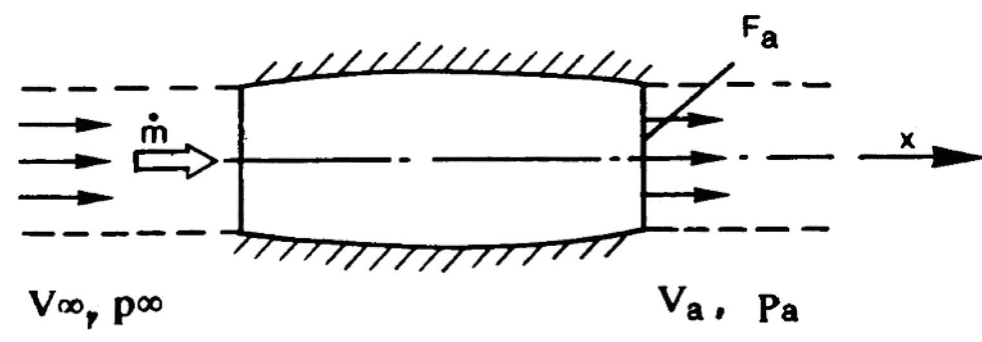
\includegraphics[width=6cm]{images/Schub.png}  
\end{center}

\subsubsection{Wirkungsgrad von Flugantrieben}

\begin{itemize}
    \item $\eta_{tot} = \eta_t \eta_p$
    \item $\eta_t =$ thermischer Wirkungsgrad (im System produzierte mechanische Energie / Wärmeenergie Treibstoff)
    \item $\eta_p =$ Vortriebswirkungsgrad (am Flugzeug nutzbare Arbeit / mechanische Energie)
\end{itemize}

\begin{center}
    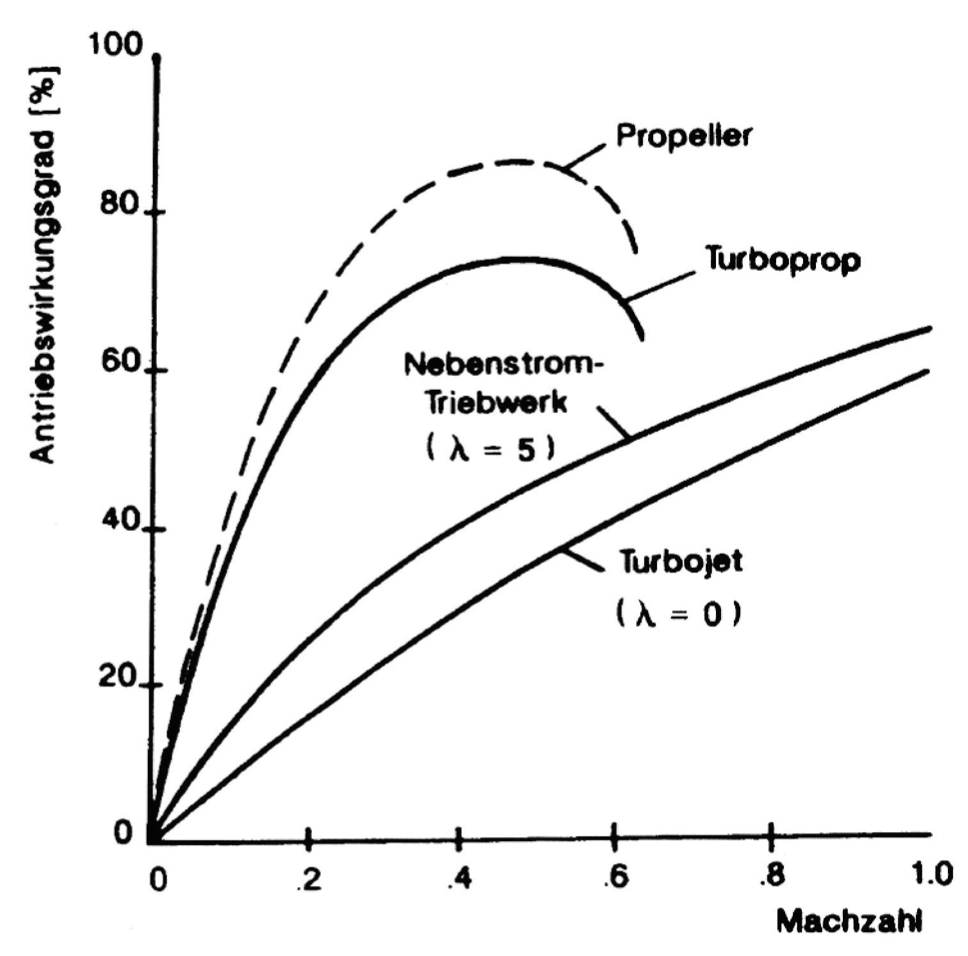
\includegraphics[width=6cm]{images/Antriebswirkungsgrade_Prop_Jet.png}
\end{center}

\subsubsection{Kolbenmotoren}

\begin{itemize}
    \item Leistung Kolbenmotor = $P = P_{IP} = \tilde{p} F_K H n N = \tilde{p} V n$
    \item $\tilde{p} = $ Mittlerer effektiver Druck, $F_K = $ Kolbenfläche, $H=$ Hub, $n=$ Drehzahl, $N=$ Anzahl Kolben, $V=$ Hubvolumen
    \item Bremsleistung = $P_{BP} = \eta_{mech} P_{IP}$
    \item Thermische Leistung = $P_{th} = \dot{w} H_{Br}$
    \item $\dot{w} =$ Brennstoffdurchlass $[\frac{kg}{s}]$, $H_{Br}=$ Heizwert $[J/kg]$
    \item $\eta_{th} = \frac{P_{BP}}{P_{th}} = \frac{P_{BP}}{\dot{w} H_{Br}} = \frac{1}{BSFC \cdot H_{Br}}$ 
\end{itemize}

Die Leistung (Vollgasleistung) hängt hauptsächlich auch von der Flughöhe ab, daher muss diese noch angepasst werden:

\begin{itemize}
    \item $P = P_0 \sqrt{\frac{T_{ISA}}{T}} [(1+c)\Theta^{4.256}-c]$
    \item $P_0 = $ Vollgasleistung in $H = 0$, ISA
    \item $T_{ISA}=$ Temperatur in $[K]$ der ISA-Atmosphäre bei Höhe $H$ 
    \item $0.1 \leq c \leq 0.3 = $ empirischer Faktor
    \item $\Theta(H) = \left[\frac{T}{T_0}\right]_{ISA} = 1-22.558\cdot 10^{-6}\cdot H$ ($H = [m]$)
\end{itemize}

Weitere Faktoren für die Motorleistung:

\begin{itemize}
    \item Luft-Treibstoff-Gemisch 
    \item Führung der Zylinder, Druck im Ansaugteil (Turbolader)
    \item Maximal zulässige Drehzahl
\end{itemize}

\subsubsection{Propeller (5.20f)}

\begin{center}
    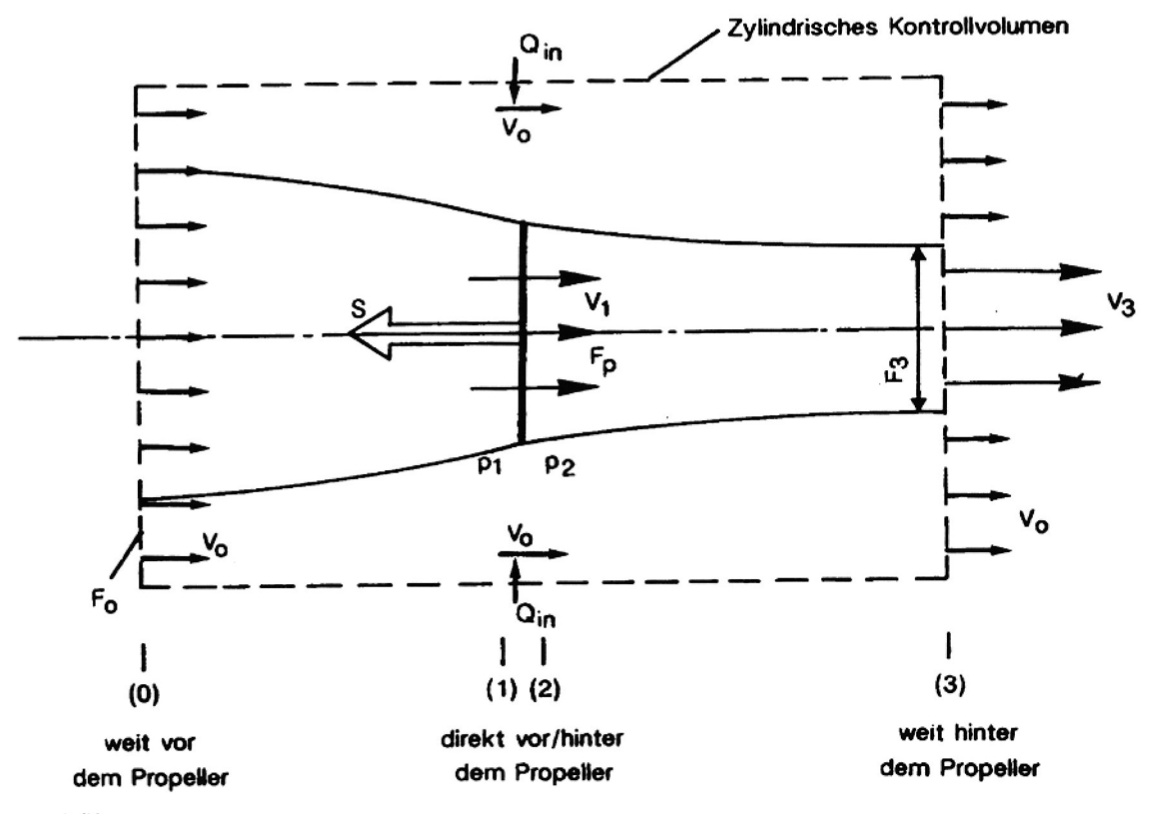
\includegraphics[width=6cm]{images/Propeller_Ideal.png}
\end{center}

Aus Impuls und Massenerhaltungsgleichungen folgt:

\begin{itemize}
    \item $S = \frac{\rho}{2} F_p (V_3^2 - V_0^2) = \rho F_p V_1 (V_3-V_0)$
    \item $S = \rho F_p (V_0 + \nu) 2\nu$ ($\nu = $ induzierte Geschwindigkeit)
    \item $\nu = -\frac{V_0}{2} + \sqrt{\left( \frac{V_0}{2}\right)^2 + \frac{S}{2\rho F_p}}$
    \item $S/F_p = $ Propellerbelastung, Schub $S$ pro Propellerfläche $F_p$
\end{itemize}

Die Leistung $P = [W]$ lässt sich dann wie folgt berechnen:

\begin{itemize}
    \item $P = S\cdot V_1 = S\cdot (V_0+\nu) = \frac{\rho}{2} F_p V_1 (V_3^2 - V_0^2) = 2 \rho F_p \nu (V_0+\nu)^2$
    \item $P_{Nutz} = S \cdot V_0$
\end{itemize}

Wirkungsgrad eines idealen Propellers:
\begin{itemize}
    \item $\eta_i = \frac{P_{Nutz}}{P} = \frac{1}{1 +\frac{\nu}{V_0}} = \frac{2}{1 + \sqrt{1 + c_s}}$
    \item Schubbeiwert $c_s = \frac{S}{\frac{\rho}{2}V_0^2 F_P}$
\end{itemize} 

\textbf{Resultate der Impulstheorie}

\begin{itemize}
    \item Bei gegebenem Schubbeiwert $c_s$ kann der Wirkungsgrad direkt berechnet werden
    \item Die Schubgrenze (für gegebene Motorleistung) folgt aus der Beziehung für die Leistung und kann in einem Schub-Leistungsdiagramm mit Fluggeschwindigkeit als Parameter dargestellt werden
\end{itemize}

\begin{center}
    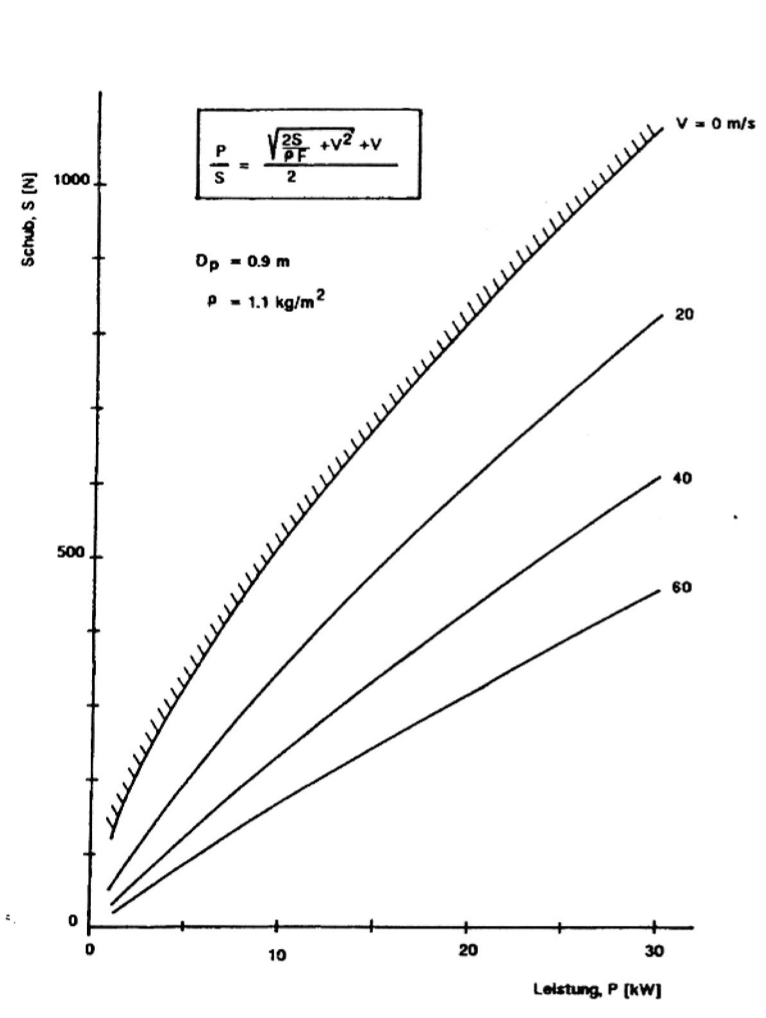
\includegraphics[width=6cm]{images/Schubgrenze.png}
\end{center}

\textbf{Berechnung des Standschubes $S_0$}

\begin{itemize}
    \item $\nu_0 = \sqrt{\frac{S_0}{2 \rho F_p}}$, falls da $V_0=0$
    \item $P_0 = S_0 \nu = \frac{S_0^{2/3}}{\sqrt{2 \rho F_p}}$
    \item $S_0 = \left( 2 \rho F_p \right)^{1/3} P_0^{2/3}$
\end{itemize}

\textbf{Abhängigkeit des Schubes von der Geschwindigkeit} \newline

Hier ist die Annahme, dass die Leistung unabhängig von der Geschwindigkeit ist, daher $P(V) = P(V_0) = P_0$

\begin{itemize}
    \item $P = \frac{S}{2}\left( V_0 + \sqrt{V_0^2 + \frac{S}{\frac{\rho}{2} F_p}}\right) = \frac{S_0^{3/2}}{\sqrt{2 \rho F_p}}$
    \item Aus Umformungen folgt folgende Gleichung:
    \item $\left( \frac{S}{S_0} \right)^3 + \left(\frac{S}{S_0} \right) \frac{V_0}{\nu_0} - 1 = 0$ (Polynom 3. Grades)
    \item Das Polynom kann numerisch ermittelt oder aus Tabellen herausgelesen werden. Die Gleichung gilt universell. Falls $S_0$ und $V_0$ gegeben sind, kann die Abhängigkeit des Schubes $S$ von $V$ berechnet werden
\end{itemize}

\subsubsection{Blattelementtheorie}

\begin{center}
    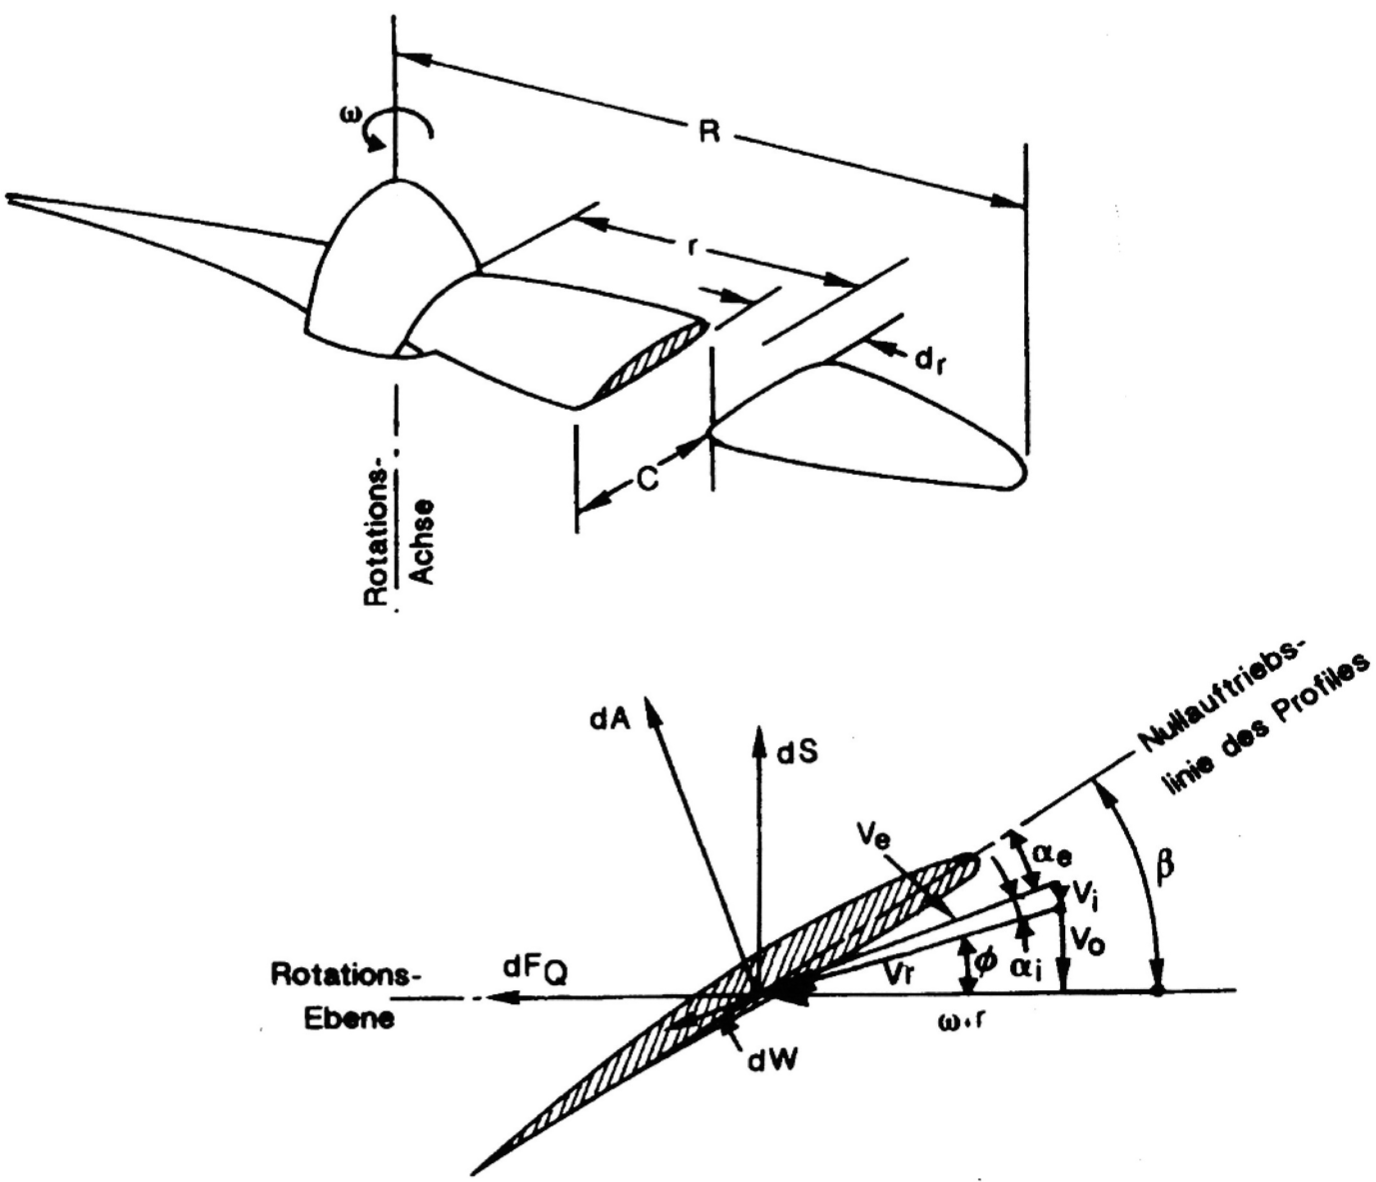
\includegraphics[width=7.5cm]{images/Blattelementtheorie_1.png}
\end{center}

\textbf{Wichtige Grössen (5.32f)}

\begin{itemize}
    \item $c_P = \frac{P}{\rho n^3 D^5} = $ Leistungsbeiwert
    \item $c_T = \frac{S}{\rho n^2 D^4} = $ Schubbeiwert
    \item $J = \frac{V_0}{n D} = $ Fortschrittsgrad
    \item $\eta = \frac{S V_0}{P} = \frac{c_T}{c_P} J = $ Propellerwirkungsgrad
\end{itemize}

Mit den gegebenen Grössen lässt sich im Propellerdiagramm (entweder fixer oder verstellbarer Propellersteigwinkel $\beta$) ablesen,
was der Propellerwirkungsgrad ist als Funktion vom Fortschrittgrad $\eta = f(J)$

\begin{enumerate}
    \item $V_0$ gegeben für Flugzeug (Fluggeschwindigkeit), $n$ ebenfalls gegeben sowie Propellerdurchmesser $D$
    \item Daraus lässt sich $J = \frac{V_0}{nD}$ bestimmen
    \item Aus dem Propellerdiagramm mit $\eta$ bei gegebenem $J$ und $\beta$ bestimmen
    \item Aus $n$ ($P = P(n)$ aus Motor-Leistungskennlinie) und $\eta$ lässt sich nun $S = \frac{\eta P}{V_0}$ bestimmen
\end{enumerate}

\subsubsection{Einbauverhältnisse}

Für Verluste durch Versperrwirkung, beispielsweise am Rumpf, sind unberücksichtigt und analytisch schwer vorherbestimmbar. Daher kann als Richtlinie gelten:

\begin{itemize}
    \item $\eta_{eff} = 0.9 \eta_{Propeller}$
\end{itemize}

Versuche in Windkanälen können hier mehr Informationen liefern, z.B. durch einen erzeugten Drall vom Propeller.

\setcounter{subsection}{11} % Initiate new counter
\subsection{Flugmesstechnik}

\subsubsection{Einsatz und Anwendung}

Auf der einen Seite beliefern Sensoren die Anzeigeinstrumente im Cockpit mit den notwendigen Informationen, damit der Pilot das Flugzeug zweckmässig führen kann. Andererseits werden Datn in Flugregler und Autopiloten geführt, um den Piloten in der Flugbahnführung und -planung, Navigation und Einhalten der Grenzwerten zu unterstützen, oder sogar zu ersetzen. Ebenso dienen flugzeuggestütze Instrumentierung bei, Flugleistungen zu ermitteln, Flugeigenschaften zu quantifizieren, Grenzwerte festzulegen. 

\subsubsection{Messung der Flughöhe}

Folgende Messmethoden dienen zur Höhenbestimmung:

\begin{itemize}
    \item Messung des Umgebungsdrucks
    \item Messung der Umgebungstemperatur
    \item Messung der Umgebungsdichte
    \item Radar-Vermessung, flugzeuggestützt
    \item Peilverfahren (Radar, GPS,...)
    \item Trägheitsnavigationssysteme
\end{itemize}

wobei die ersten drei die Eigenschaften der Atmosphäre genutzt wird. Im allgemeinen ist die barometrische Höhenmessung auch heute die noch am weitesten verbreitete Methode. Die \textbf{Druckmessstellen} sind folgende, welche in Frage kommen:

\begin{itemize}
    \item statische Druckbohrung am Rumpf
    \item statische Drucksonde, in Kombination mit Gesamtdruckmessung (Prandtl-Sonde)
    \item Kabineninnendruck bei Flugzeugen ohne Druckkabine (sehr ungenau, nur im Notfall)
\end{itemize}

Der \textbf{abgegriffene Druck ist abhängig von}:

\begin{itemize}
    \item Position der Messung
    \item Fluggeschwindigkeit
    \item Flugzeuglage relativ zur Anströmungsrichtung
    \item Regen und Vereisung
    \item Verschmutzung der Messstelle
    \item Lokale Effekte von Proprellerstrahl, Verdichtungsstössen (hohe Machzahl)
\end{itemize}

Die angabe der Druckhöhe (pressure altitude) ist die am meisten verwendete Methode. Hierzu braucht es aber ebenfalls \textbf{Einstellungen}, welche an verschidenen Orten durchgeführt werden müssen:

\begin{itemize}
    \item Höhe über Meer (QNH): Vor dem Startwird die Höhenmessanzeige auf die topographische Höhe des Flugplatzes eingestellt
    \item Höhe über Flugplatz (QFE): Vor de Start wird die Höhenmessanzeige auf $0$ gestellt
    \item Standard-Einstellung (QNE): Der Höhenmesser wird so eingestellt , dass bei $1013~Pa$ eine Höhe von $0~m$ angezeigt wird
\end{itemize}

\subsubsection{Messung der Fluggeschwindigkeit}



\subsubsection{Messung der Strömungsrichtung}

Nebst Staudruck ist die Richtung der Anströmung ebenfalls eine wichtige aerodynamische Grösse. Insbesondere ist man interessiert an den Werten des Anstell- ($\alpha$) und Schiebewinkels ($\beta$). In Transportflugzeugen wird lediglich der Anstellwinkel gemessn, jedoch bei Kampfflugzeugen auch der Schiebewinkel. \newline 
\newline Somit werden lokale Strömungswinkel am Ort von der Sonde gemessen. Der gemessene Winkel entspricht beispielsweise nicht exakt dem
Anstellwinkel des Flugzeugs. Der Zusammenhang wird mittels Eichung (Windkanal- oder Flugversuch) ermittelt. \newline
\newline Der grosse Vorteil der Strömungsrichtungmessung liegt darin, dass direkt aerodynamische Grössen ermittelt werden (unabhängig von Druck, Temperatur, Masse etc.) im Gegensatz zur Geschwindigkeitsmessung. \newline
\newline Die Strömungsrichtungsmessung ist vielfach nur eine Hilfsfunktion und ist für die Flugsicherheit nicht von primärer Bedeutung. 

\subsection*{Disclaimer}

Diese Zusammenfassung basiert auf den persönlichen Notizen und Zusammenfassungen früherer Jahre. Fehler sind unvermeidbar und es besteht keine Garantie dass diese Zusammenfassung vollständig komplett ist. 

\end{multicols*}
\end{document}

